\section{Short Description Of The Protocol} % Major section

\subsection{SSL Handshake}
\begin{wrapfigure}{R}{0.4\textwidth}
	\vspace{-30pt}
  \begin{center}
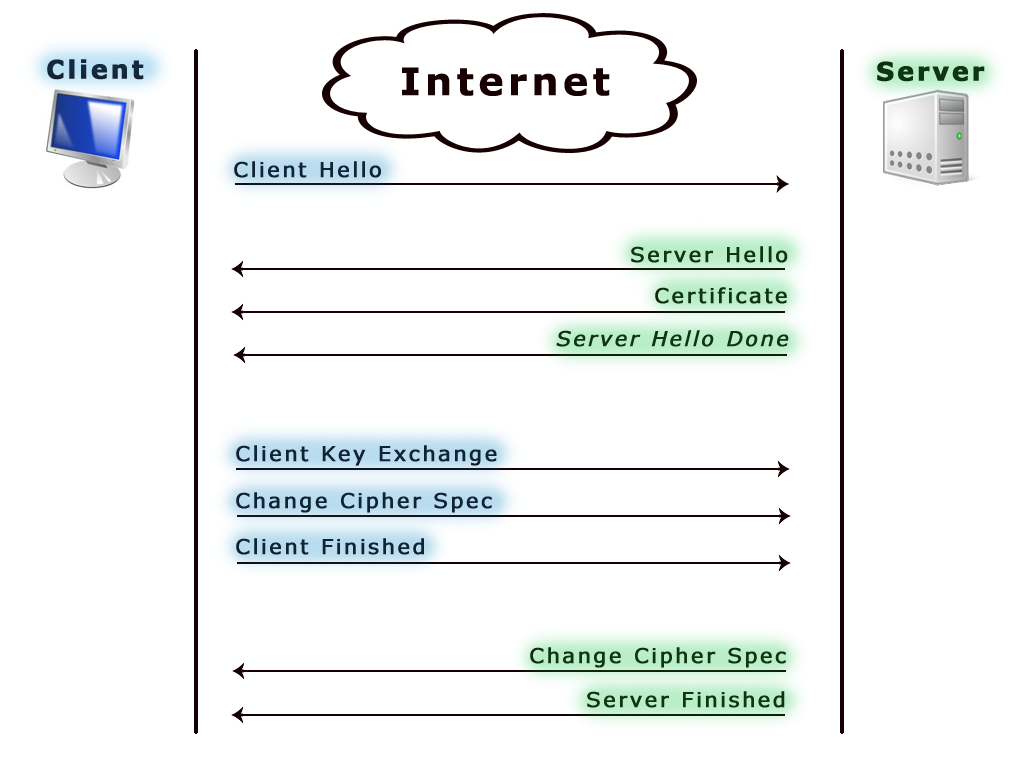
\includegraphics[width=0.50\textwidth]{SSL_handshake_image}
  \end{center}
	\vspace{-20pt}
  \caption{SSL Handshake}
\end{wrapfigure}
When you visit a website using the https protocol~\cite{wikipediaHTTPS} \textit{(technically not a protocol, since SSL/TLS is just layered on top of the HTTP protocol)}, the client and the webserver tries to establish a secure connection using SSL/TLS~\cite{wikipediaSSLTLS}. But before the secure connection is established, we have to perform a SSL handshake.\\ 
However, in order to complete a SSL handshake, the client and the server has to complete a number of steps, some of which are optional. And if for some reason a problem occurs in the negotiation, the connection is usually dropped.\\\\
In this section we will give a brief overview of how the SSL handshake is completed and how it makes your communication with the web server secure.

\subsubsection{9 Steps To Secure Communication}
\begin{enumerate}
\item The client sends a ClientHello message to the server. This message contains information about which version the client supports, some randomly generated data and a list of all the cipher suites the client supports.
\item The server will now respond with a Server Hello message which include the highest version number both sides support, some randomly generated data and the cipher suite chosen by the server. It is worth mentioning that the cipher suite chosen by the server is the strongest suite both sides supports.
\item Now the server will send its certificate to the client. The server's public key is stored inside this certificate, and is used by the client to authenticate and encrypt the premaster key.
\item At this point the server is done, and waits for a response from the client.
\item It is now time to start exchanging keys. In step 1 and 2 both the client and the server sent some random values to each other. These random values is now used to generate the premaster secret. After the premaster secret is generated, it is encrypted using the server's public key and sent back to the server.
\item The client now sends a Change Cipher Spec message to the server, which basically says that all data being sent from the client from now on will be encrypted.
\item To finish the negotiation from the client's side, a Client Finished message is sent to the server.
\item The server now respond with a Change Cipher Spec message and tell the client that all data sent from the server from now on will be encrypted.
\item To complete the negotiation the server sends a Server Finished message back to client. And if everything went well the SSL handshake is now finished and a secure channel is initiated between the client and the server.
\end{enumerate}
This is obviously a very brief overview of how the SSL handshake works. But in section 4, Bit-Level Description, we will go into more detail about the handshake, and also explain exactly what kind of data and values are being transmitted from the client to the server, and vice versa.